\chapter{Engine Diagram}

% All this appendix uses make syntax
% \lstset{language=make}

%\section{Makefile.test}

%\lstset{caption=Testing Targets Makefile (Makefile.test), label=lst:makefile-test}
%\lstinputlisting{src/code/build/Makefile.test}
\begin{center}
	\begin{figure}[here!]
		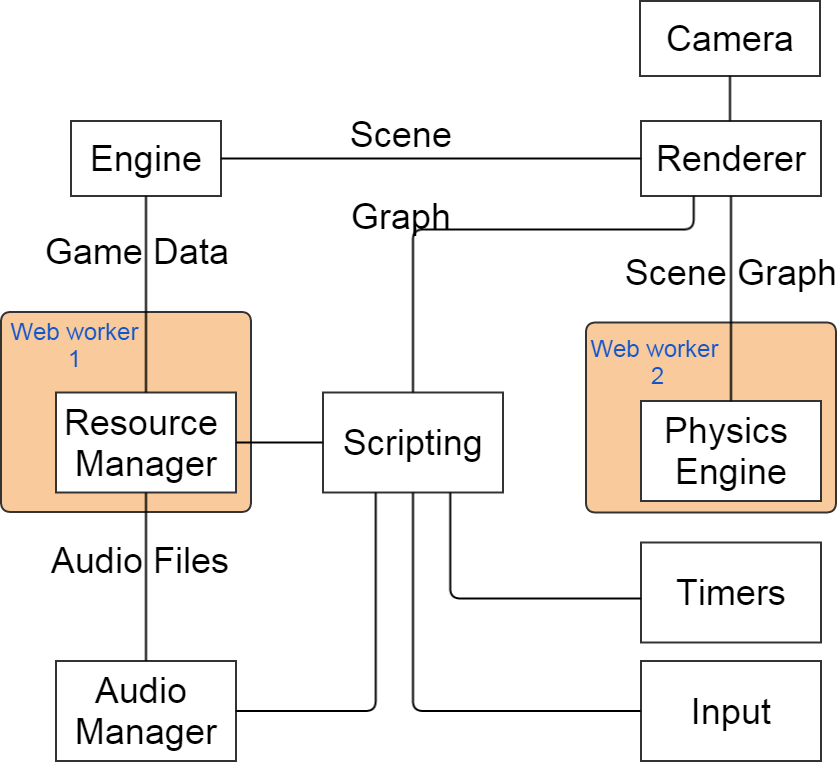
\includegraphics[width=\textwidth]{src/img/engine-diagram.png}
%		\caption{Engine Diagram}
		\label{img:engine}
	\end{figure}
\end{center}


\chapter{Renderings}

\begin{center}
	\begin{figure}[here!]
		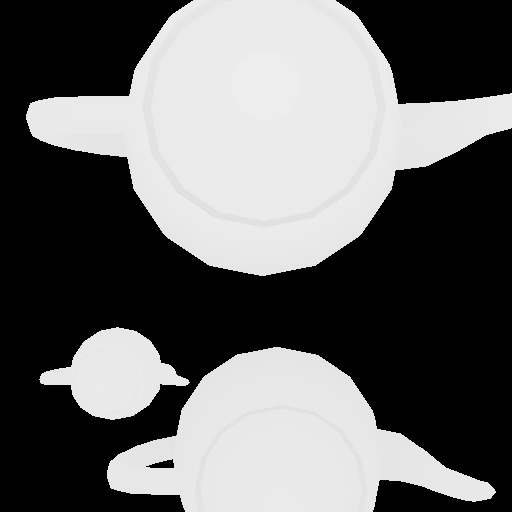
\includegraphics[width=\textwidth]{src/img/screenshots/depth.png}
		\caption{Depth Buffer in view space}
		\label{img:depth}
	\end{figure}
\end{center}
\begin{center}
	\begin{figure}[here!]
		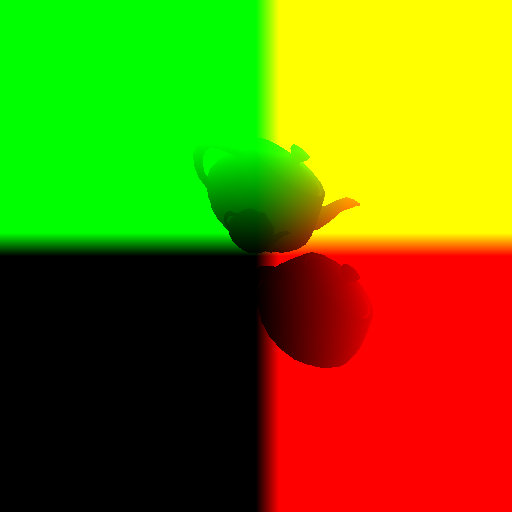
\includegraphics[width=\textwidth]{src/img/screenshots/view-space.png}		\caption{View space positions}
		\label{img:view-space}
	\end{figure}
\end{center}

\begin{center}
	\begin{figure}[here!]
		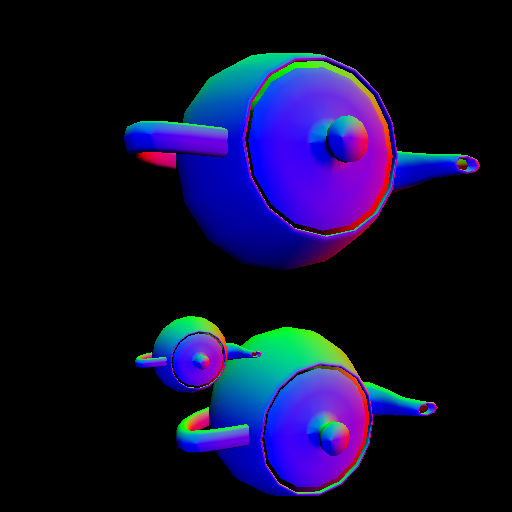
\includegraphics[width=\textwidth]{src/img/screenshots/normals.png}		\caption{Normals}
		\label{img:normals}
	\end{figure}
\end{center}